\section{Algorytm Kruskala}
\subsection{Pseudokod opisujący działanie algorytmu Kruskala:}

\textbf{Inicjalizacja:}
\begin{enumerate}
	\item	Utwórz las L z wierzchołków oryginalnego grafu – każdy wierzchołek jest na początku osobnym drzewem.
	\item Utwórz posortowany zbiór S zawierający wszystkie krawędzie oryginalnego grafu.
\end{enumerate}

\begin{center}
	\textbf{Tworzenie MST}
\end{center}

\begin{enumerate}
\item Wybierz i usuń z S jedną z krawędzi o minimalnej wadze.
\item Jeśli krawędź ta łączyła dwa różne drzewa, to dodaj ją do lasu L tak, aby połączyła dwa odpowiadające drzewa w jedno.
\item W przeciwnym wypadku odrzuć ją.
\item Jeżeli wciąż istnieje więcej niż jedno drzewo przejdź do punktu 1.
\end{enumerate}

Po zakończeniu algorytmu L jest minimalnym drzewem rozpinającym zgodnie z \cite{gis}.

\newpage
\subsection{Działanie algorytmu na przykładzie}
Dany jest graf posiadający następujące składowe:
\begin{itemize}
\item Wierzchołki: {A}, {B}, {C}, {D}, {E}
\item Krawędzie: {A B, 1}, {A D, 1}, {C D, 1}, {D E, 1}, {B C, 1}, {A C, 5}, {C E, 5}
\end{itemize}

\textbf{Legenda oznaczeń w poniższym przykładzie:}\\
\begin{figure}[htb!]
	\centering
	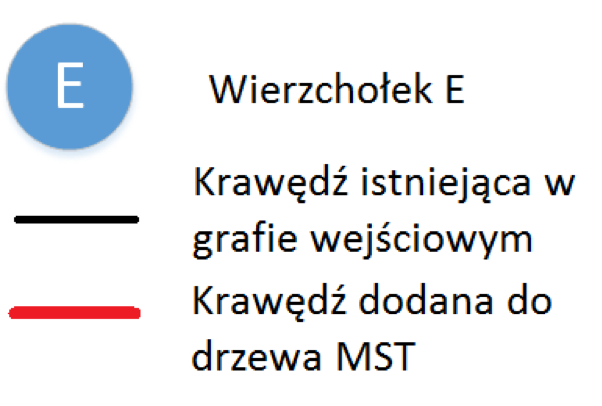
\includegraphics[width=0.3\textwidth]{tex/fig/Picture1}
	\caption{Oznaczenia wykorzystane w opisie algorytmu Kruskala}
	\label{fig: legendK}
\end{figure}

\begin{center}
	\textbf{Przebieg algorytmu}
\end{center}
\begin{enumerate}
	\item Pierwszy etap wykonania algorytmu - ustalenie zbioru wierzchołków S oraz zbioru krawędzi L:\\
	S: {A}, {B}, {C}, {D}, {E}
\\
	L: {A B}, {A D}, {C D}, {D E}, {B C}, {A C}, {C E}
\\
	\begin{figure}[htb!]
		\centering
		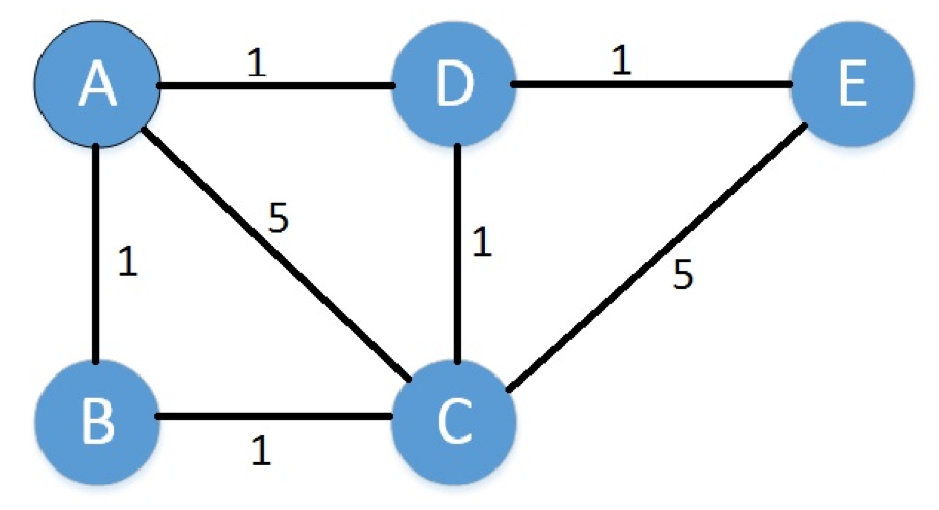
\includegraphics[width=0.4\textwidth]{tex/fig/Picture2}
		\caption{Przykładowy graf / pierwszy etap wykonania algorytmu Kruskala}
		\label{fig: legendK1}
	\end{figure}

\newpage
\item Krok 2\\
Ze zbioru S usunięta została jedna z krawędzi o najmniejszej wadze. {A B} Ponieważ wierzchołki, które łączyła znajdowały się w osobnych drzewach w L zostały połączone w jedno drzewo {A, B}, więc dodawana jest krawędź dodawana jest do W.\\
S: {A, B}, {C}, {D}, {E}
\\
L: {A D}, {C D}, {D E}, {B C}, {A C}, {C E}
\\
	\begin{figure}[htb!]
	\centering
	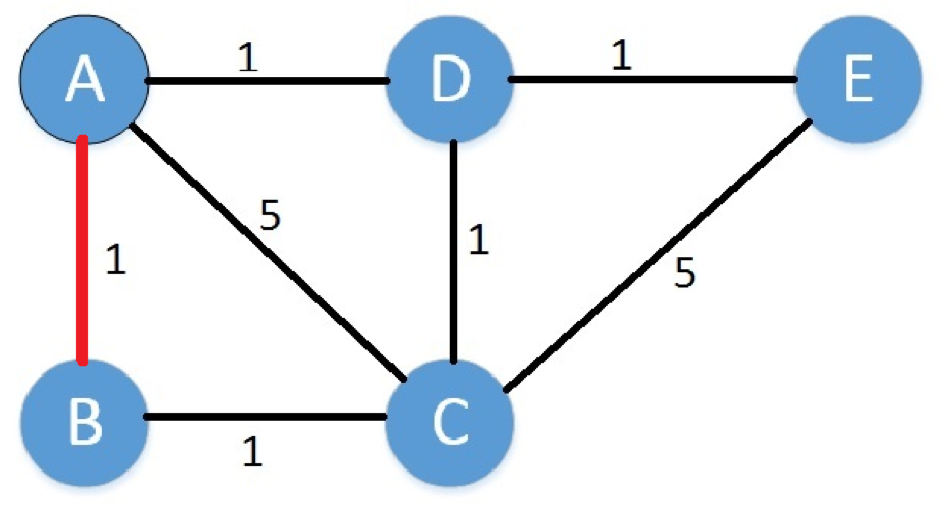
\includegraphics[width=0.4\textwidth]{tex/fig/Picture3}
	\caption{Drugi etap wykonania algorytmu Kruskala}
	\label{fig: legendK2}
\end{figure}

\item Krok 3\\
Ze zbioru S usunięta została jedna z krawędzi o najmniejszej wadze. {A D} Ponieważ wierzchołki, które łączyła znajdowały się w osobnych drzewach w L zostały połączone w jedno drzewo {A, B, D}, więc dodawana jest krawędź dodawana jest do W.\\
S: {A, B, D}, {C}, {E}
\\
L: {C D}, {D E}, {B C}, {A C}, {C E}
\\
	\begin{figure}[htb!]
	\centering
	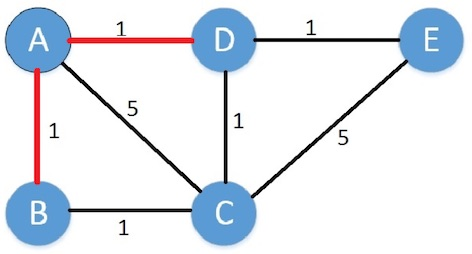
\includegraphics[width=0.4\textwidth]{tex/fig/Picture4}
	\caption{Trzeci etap wykonania algorytmu Kruskala}
	\label{fig: legendK3}
\end{figure}
\newpage
\item Krok 4\\
Ze zbioru S usunięta została jedna z krawędzi o najmniejszej wadze. {C D} Ponieważ wierzchołki, które łączyła znajdowały się w osobnych drzewach w L zostały połączone w jedno drzewo {A, B, C, D}, więc dodawana jest krawędź dodawana jest do W.\\
S: {A, B, C, D}, {E}
\\
L: {D E}, {B C}, {A C}, {C E}
\\

\begin{figure}[htb!]
	\centering
	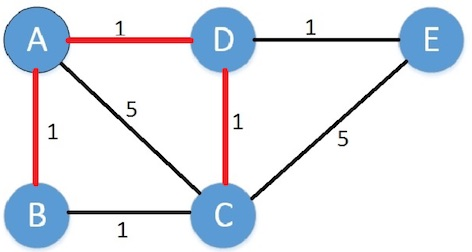
\includegraphics[width=0.4\textwidth]{tex/fig/Picture5}
	\caption{Czwarty etap wykonania algorytmu Kruskala}
	\label{fig: legendK4}
\end{figure}

\item Krok 5\\
Ze zbioru S usunięta została jedna z krawędzi o najmniejszej wadze. {D E} Ponieważ wierzchołki, które łączyła znajdowały się w osobnych drzewach w L zostały połączone w jedno drzewo {A, B, C, D, E}, więc dodawana jest krawędź dodawana jest do W. Ponieważ w zbiorze L pozostał tylko jeden zbiór wykonanie algorytmu zostaje zakończone.\\
S: {A, B, C, D, E}
\\
L: {B C}, {A C}, {C E}
\\
\begin{figure}[htb!]
	\centering
	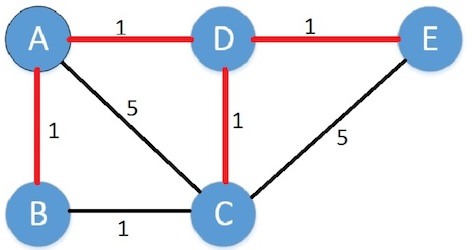
\includegraphics[width=0.4\textwidth]{tex/fig/Picture6}
	\caption{Piąty etap wykonania algorytmu Kruskala – uzyskane MST}
	\label{fig: legendK5}
\end{figure}

\textbf{Jak widać nie zawiera ono żadnych cykli i zawiera tylko krawędzie o minimalnej wadze.}\\
\end{enumerate}
\newpage
\subsection{Opis struktur danych i algorytmów}
\begin{itemize}
		\item Dane zostaną pobrane z pliku tekstowego o ustalonym formacie.
		\item Ponieważ samodzielna implementacja podstawowych algorytmów mija się z celem użyta zostanie jedna z funkcji bibliotecznych języka JAVA.
		\item Wykrywanie cykli oraz scalanie odbywać się będzie poprzez użycie struktury zbiorów rozłącznych - \cite{gis2}.
		\item Krawędzie dodane do grafu będą wpisywane do listy w celu zapisania uzyskanego rozwiązania.
\end{itemize}
